\section{Theorie}
Das Ziel dieses Versuches ist es, die Kristallstruktur und die Größe der Einheitszelle
von zwei verschiedenen Probematerialien zu bestimmen, indem Debye-Scherrer-Aufnahmen
angefertigt werden.

\subsection{Beschreibung von Kristallstrukturen}
Ein Großteil der kondesierten Materie liegt in kristalliner Struktur vor.
Um dieser Struktur aufzulösen, muss die räumliche Auflösung des Messgeräts in der
gleichen Größenordnung liegen wie die Abstände zwischen den Atomen. Dafür eignen sich
neben langsamen Neutronen oder Elektronen auch Röntgenstrahlen. Die im folgenden
beschriebene Methode basiert auf der Beugung dieser Röntgenstrahlung an der Kristallstruktur.

Die räumliche Beschreibung der Kristalle lässt sich aus zwei Elementen zusammensetzen:
der Basis und des Punktgitters. Zusammen ergeben sie die Kristallstruktur, wie in
\autoref{abb:struktur} dargestellt.
\begin{figure}
  \centering
  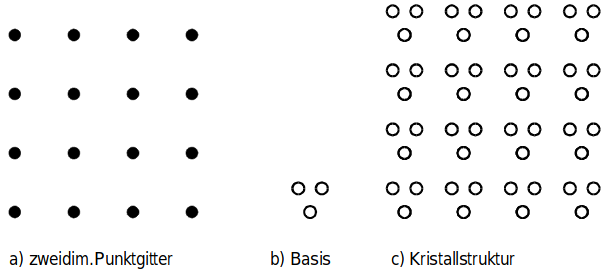
\includegraphics[scale=0.5]{content/pics/basis_gitter.png}
  \caption{Bestandteile der Kristallstruktur. \cite{anleitung}}
  \label{abb:struktur}
\end{figure}
Die Basis besteht dabei entweder aus einem Atom oder einer Atomgruppe. Um die verschiedenen
Punktgitter zu klassifizieren, werden durch drei Vektoren $\vec{a}, \vec{b}$ und $\vec{c}$
fundamentale Translationen aufgespannt, die durch
\begin{equation}
  \vec{t} = n_1 \, \vec{a} + n_2 \, \vec{b} + n_3 \ \vec{c} \qquad \text{mit} \ n_i \in \mathbb{N}
  \label{eqn:1}
\end{equation}
definiert sind. Mithilfe dieser Vorschrift lässt sich das ganze Gitter aufspannen, da
alle Punkte, die sich mit \eqref{eqn:1} darstellen lassen, Gitterpunkte sind.

Ein weitere Größe, die bei der Beschreibung von Kristallstrukturen von Bedeutung
ist, ist die Elementarzelle.  Diese ist definiert als die kleinste Einheit, durch
welche die Kristallstruktur vollständig festgelegt ist. Falls in dem von den Vektoren
aus \eqref{eqn:1} aufgespannte Parallelepiped nur in den acht Eckpunkten Atome sitzen,
dann ist diese Elementarzelle primitiv. Sie enthält nur ein Atom. Allerdings lässt sich
die Kristallstruktur nicht mehr vollständig aus vielen primitiven Elementarzellen
aufbauen, falls die Basis aus mehr als einem Atom besteht, da in diesem Fall die Atome
nicht nur in den Eckpunkten des Parallelepipeds sitzen.

Im nachfolgenden Versuch werden verschiedene kubische Strukturen untersucht.
Eine davon ist die kubisch-raumzentrierte Struktur (\textit{eng.} bcc (body centered cubic)).
Diese besitzt zwei Atome pro Elementarzelle. Eine Darstellung ist in \autoref{abb:elementarzelle_kubisch}
zu finden.
\begin{figure}
  \centering
  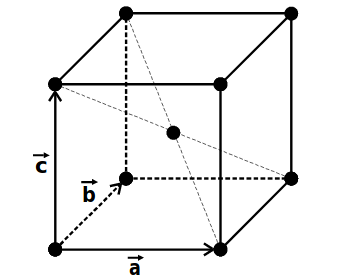
\includegraphics[scale=0.5]{content/pics/elementarzelle_kubisch.png}
  \caption{Schematische Darstellung der Elementarzelle des kubisch-raumzentrierten
  Gitters. \cite{anleitung}}
  \label{abb:elementarzelle_kubisch}
\end{figure}
Im Koordinatensystem der Elementarzelle liegen die Atome bei
\begin{equation}
  (0, 0, 0) \ \text{und} \ (\frac{1}{2}, \frac{1}{2}, \frac{1}{2}) \, .
  \label{eqn:atome-raumzentriert}
\end{equation}
Die acht nächsten Nachbarn haben einen Abstand untereinander von
$\frac{1}{2} \sqrt{3} a$, mit $a$ als Kantenlänge des Würfels.

Im Gegensatz zur kubisch-raumzentrierten Struktur gibt es bei der kubisch-flächenzentrierten
(\textit{eng.} fcc (face centered cubic)) Struktur statt des zentralen Atoms in der
Mitte des Würfels jeweils ein Atom in der Mitte der Seitenflächen des Würfels, wie
in \autoref{abb:elementarzelle_flaeche} zu sehen.
\begin{figure}
  \centering
  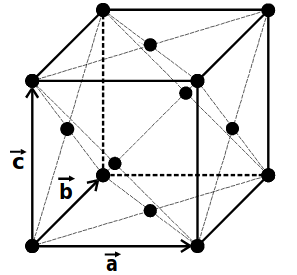
\includegraphics[scale=0.5]{content/pics/elementarzelle_flaeche.png}
  \caption{Schematische Darstellung der Elementarzelle des kubisch-flächenzentrierten
  Gitters. \cite{anleitung}}
  \label{abb:elementarzelle_flaeche}
\end{figure}
Die Atome der Elementarzelle liegen bei
\begin{equation}
  (0, 0, 0), (\frac{1}{2}, \frac{1}{2}, 0), (\frac{1}{2}, 0, \frac{1}{2}) \ \text{und}
  \ (0, \frac{1}{2}, \frac{1}{2}) \, .
  \label{eqn:atome-flaechenzentriert}
\end{equation}
Die zwölf nächsten Nachbarn haben einen Abstand von $\frac{1}{2} \sqrt{2} a$
untereinander.
% cleares the page and appends all not yet used floats at the beginning of the
% next page
\pagebreak
\subsection{Millersche Indizes und Abstandsberechung}

Eine wichtige Größe für diesen Versuch sind die Millerschen Indizes. Diese kennzeichnen
die Lage der Netzebenen im Kristall relativ zum Koordinatensystem des Kristalls,
welche definiert sind als Ebene, in der die Schwerpunkte der Atome liegen.
Die Millerschen Indizes, meist mit h, k und l bezeichnet, sind die Zahlenwerte,
die sich errechnen, wenn die Schnittpunkte der Netzebene mit den Koordinatenachsen
gebildet und die reziproken Werte genommen werden. Um gebrochenen Zahlen zu vermeiden,
wird das Zahlentripel mit den Inversen der gebrochenen Zahlen multipliziert. Nach
Definition werden negative Achsenabschnitte durch einen Strich über dem jeweiligen Index
gekennzeichnet. Falls eine Netzebene parallel zu einer Achse liegt, dann ist der Millersche
Index 0, da der Schnittpunkt mit der Koordinatenachse im Unendlichen liegt.

Die Millerschen Indizes sind unter anderem deswegen eine zentrale Größe in der Beschreibung
von Kristallstrukturen, da aus ihnen relativ einfach der Abstand benachbarter Netzebenen
berechnen lässt. In \autoref{abb:abstand} ist eine Skizze zur Berechnung zu sehen.
\begin{figure}
  \centering
  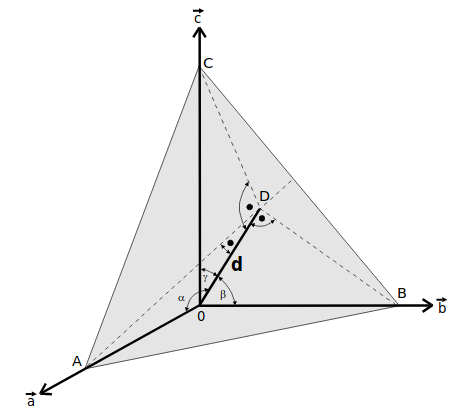
\includegraphics[scale=0.5]{content/pics/netzebenenabstand.png}
  \caption{Grafische Darstellung der wichtigsten Größen zur Berechnung des Netzebenenabstandes
  aus den Millerschen Indizes. \cite{anleitung}}
  \label{abb:abstand}
\end{figure}
Da der Netzebenabstand $d$ senkrecht auf den beiden Netzebenen(eine mit den Punkten
A, B und C und eine mit dem Ursprung), sind die Dreiecke ODA, ODB und ODC rechtwinklig.
Aus trigonometrischen Beziehungen ergibt sich
\begin{equation}
  d = \left(\sqrt{\frac{h^2}{a^2} + \frac{k^2}{b^2} + \frac{l^2}{c^2}}\right)^{-1}
  \label{eqn:abstand}
\end{equation}
und für kubische Systeme mit $a = b = c$ wird \eqref{eqn:abstand} zu
\begin{equation}
  d = \frac{a}{\sqrt{h^2 + k^2 + l^2}} \, .
  \label{eqn:abstand_kubisch}
\end{equation}
\pagebreak
\subsection{Beugung von Röntgenstrahlen an Kristallen}

\section{Durchführung}
\subsection{Aufbau}
\subsection{Versuchsdurchführung}
